
\documentclass{beamer}[10]
% \documentclass[handout]{beamer}[10]
\usepackage{pgf}
\usepackage[danish]{babel}
\usepackage[utf8]{inputenc}
\usepackage{beamerthemesplit}
\usepackage{graphics,epsfig, subfigure}
\usepackage{url}
\usepackage{srcltx}
\usepackage{hyperref}
\usepackage{bookmark}
\usepackage{nicefrac}
\usepackage{multicol}
\usepackage{vwcol}
\usepackage{microtype}
\usepackage[all]{xy}
\usepackage{amssymb}


\definecolor{kugreen}{RGB}{50,93,61}
\definecolor{kugreenlys}{RGB}{132,158,139}
\definecolor{kugreenlyslys}{RGB}{173,190,177}
\definecolor{kugreenlyslyslys}{RGB}{214,223,216}
\setbeamercovered{invisible}
\mode<presentation>
\usetheme[numbers,totalnumber,compress,sidebarshades]{PaloAlto}
\setbeamertemplate{footline}[frame number]

  \usecolortheme[named=kugreen]{structure}
  \useinnertheme{circles}
  \usefonttheme[onlymath]{serif}
  \setbeamercovered{invisible}
  \setbeamertemplate{blocks}[rounded][shadow=true]

\logo{
\includegraphics[width=0.8cm]{KULogo}}
%\useoutertheme{infolines} 
\title{Equations in Hyperbolic(-esque) Groups}
\author{Barak Ohana}
\institute{The Hebrew University of Jerusalem}
\date{9 Sep 2024}

\newcommand{\sol}{\text{V}_{\Gamma}}
\renewcommand{\hom}{\text{Hom}}

%mathcal

\newcommand{\cala}{\mathcal{A}}
\newcommand{\calb}{\mathcal{B}}
\newcommand{\calc}{\mathcal{C}}
\newcommand{\cald}{\mathcal{D}}
\newcommand{\cale}{\mathcal{E}}
\newcommand{\calf}{\mathcal{F}}
\newcommand{\calg}{\mathcal{G}}
\newcommand{\calh}{\mathcal{H}}
\newcommand{\cali}{\mathcal{I}}
\newcommand{\calj}{\mathcal{J}}
\newcommand{\calk}{\mathcal{K}}
\newcommand{\call}{\mathcal{L}}
\newcommand{\calm}{\mathcal{M}}
\newcommand{\caln}{\mathcal{N}}
\newcommand{\calo}{\mathcal{O}}
\newcommand{\calp}{\mathcal{P}}
\newcommand{\calq}{\mathcal{Q}}
\newcommand{\calr}{\mathcal{R}}
\newcommand{\cals}{\mathcal{S}}
\newcommand{\calt}{\mathcal{T}}
\newcommand{\calu}{\mathcal{U}}
\newcommand{\calv}{\mathcal{V}}
\newcommand{\calw}{\mathcal{W}}
\newcommand{\calx}{\mathcal{X}}
\newcommand{\caly}{\mathcal{Y}}
\newcommand{\calz}{\mathcal{Z}}

%mathbb
\usepackage{amsfonts}
\renewcommand{\aa}{\mathbb{A}}
\newcommand{\bb}{\mathbb{B}}
\newcommand{\cc}{\mathbb{C}}
\newcommand{\dd}{\mathbb{D}}
\newcommand{\ee}{\mathbb{E}}
\newcommand{\ff}{\mathbb{F}}
\renewcommand{\gg}{\mathbb{G}}
\newcommand{\hh}{\mathbb{H}}
\newcommand{\ii}{\mathbb{I}}
\newcommand{\jj}{\mathbb{J}}
\newcommand{\kk}{\mathbb{K}}
\renewcommand{\ll}{\mathbb{L}}
\newcommand{\mm}{\mathbb{M}}
\newcommand{\nn}{\mathbb{N}}
\newcommand{\oo}{\mathbb{O}}
\newcommand{\pp}{\mathbb{P}}
\newcommand{\qq}{\mathbb{Q}}
\newcommand{\rr}{\mathbb{R}}
\renewcommand{\ss}{\mathbb{S}}
\renewcommand{\tt}{\mathbb{T}}
\newcommand{\uu}{\mathbb{U}}
\newcommand{\vv}{\mathbb{V}}
\newcommand{\ww}{\mathbb{W}}
\newcommand{\xx}{\mathbb{X}}
\newcommand{\yy}{\mathbb{Y}}
\newcommand{\zz}{\mathbb{Z}}

%parentheses
\newcommand*{\rb}[1]{\left( #1 \right)}
\renewcommand*{\sb}[1]{\left[ #1 \right]}
\newcommand*{\cb}[1]{\left\{ #1 \right\}}
\newcommand*{\ab}[1]{\left< #1 \right>}
\newcommand*{\nb}[1]{\lVert #1 \rVert}
\newcommand{\size}[1]{\left| #1 \right|}

\newcommand*{\by}{\pmb{Y}}
\DeclareMathOperator{\diam}{diam}
\DeclareMathOperator{\mcg}{MCG}
\newcommand{\sker}{\underset{\rightarrow}{\ker}}
\newcommand{\onto}{\twoheadrightarrow}
\DeclareMathOperator{\cay}{Cay}
\newcommand{\acts}{\curvearrowright}

\graphicspath{ {images/} }



\begin{document}
\frame{\titlepage \vspace{-0.5cm}}

% \frame
% {
% \frametitle{Overview}
% \tableofcontents%[pausesection]
% }

\section{First section}

\frame{
    \frametitle{Equations in Groups}
    \pause
    Let $\Gamma$  be a group,\pause and let $\Sigma\left(x_{1},\ldots,x_{d}\right)$ a (possibly infinite) system of equation on d variables. \pause
    We define the \textbf{set of solution of $\Sigma$ in $\Gamma$} to be the set
    \begin{equation*}
        \sol\left(\Sigma\right)=\left\{ \left(g_{1},\ldots,g_{d}\right)\in\Gamma^{d}\mid\Sigma\left(g_{1},\ldots,g_{d}\right)=_{\Gamma}1\right\} 
    \end{equation*}

            \pause

    There is an equivalence
    \begin{equation*}
        \sol\rb{\Sigma} \leftrightarrow \hom\rb{\nicefrac{\ff_d}{\ab{\ab{\Sigma}}}, \Gamma}
    \end{equation*}

    \pause

    So instead of studying solutions in $\Gamma$ we will study homomorphisms to $\Gamma$.

}


\subsection{Sample subsection}

\frame{

\frametitle{Sample Frame Title No. 2}

\begin{definition}
    A group $\Gamma$ is called equationally noetherian if  every set of equation is equivalent to a finite subset of it. \pause i.e. if for any set of equation $\Sigma$ there exists a finite subset $\Sigma_0$ such that $\sol\rb{\Sigma} = \sol\rb{\Sigma_0}$.
\end{definition}
\pause
\begin{example}\pause
    \begin{multicols}{2}
    \begin{itemize}
        \item All finite Groups \pause
        \item All linear groups\pause
            \begin{itemize}
                \item Thus all free groups\pause
            \end{itemize}
        \item Hyperbolic groups\\\pause
        \item[] 
        \item Free product of equationally noetherian groups\pause
        \item Groups hyperbolic relative to equationally noetherian
    \end{itemize}
    \end{multicols}
\end{example}

}

\section{Limit groups}



\frame{
    \frametitle{Limit group}
\pause 
    \begin{definition}\pause
        Let $\Gamma$ be a f.g. \pause  and $\rb{\varphi_n} \in \hom\rb{G,\Gamma}$ for some f.g. group $G$. \pause
        We define the \textbf{stable kernel} of $\rb{\varphi_n}$ to be
        \begin{equation*}
            \sker{\varphi_n} = \cb{g\in G \mid \varphi_n \rb{g} \text{is eventually } 1}
        \end{equation*}
        And e define the corrsponding \textbf{limit group} by $L=\nicefrac{G}{\sker{\varphi_n}}$
    \end{definition}
    \pause
    \begin{lemma}
        Let $\Gamma$ be a group then the following are equivalent:

        \begin{itemize}
            \item $\Gamma$ is equationally noetherian
            \pause \item For any f.g. $G$ and any $\rb{\varphi_n} \in \hom\rb{G,\Gamma}$, \pause $\varphi_n$ eventually factor through the
            quotient $G\onto L$
        \end{itemize}

    \end{lemma}
}

\frame{

    Let $\Gamma$ be a f.g. hypebolic group, meaning its caylel graph is hyperbolic.
    
    \pause Let $\rb{\varphi_n} \in \hom\rb{G,\Gamma}$. 
    
    \pause We want to show that $\varphi_n$ eventually factors through $L$.
    
    \pause Denote 
    \begin{equation*}
        \nb{\varphi_n} = \max_{s\in S} d_\Gamma \rb{1,\varphi_n\rb{ s }}
    \end{equation*}\pause
    i.e. the maximal lenght of the images of the generators of $G$ under $\varphi_n$.\pause
    \begin{fact}
        If $\nb{\varphi_n}$ is a bounded sequence then $\varphi_n$ has finitely many options (as morphisms).
    \end{fact}

}

\frame{
    Assume that $\nb{\varphi_n}$ is not bounded.
    Define at the sequence of matric spaces 
    \begin{equation*}
        X_n = \frac{1}{\nb{\varphi_n}} \cay \rb{ \Gamma } \pause  ; d_n \rb{ x,y }=\frac{1}{\nb{\varphi_n}} d_{\cay \rb{ \Gamma }} \rb{x,y}
    \end{equation*}
    \pause The rescaling of the cayley graph of $\Gamma$. \pause Now one can look at the asymptotic cone of the $X_n$'s \pause
    \begin{equation*}
                T=\lim X_n = \nicefrac{\cb{\sb{x_n} \mid x_n\in X_n}}{\ab{\sb{x_n}\sim\sb{y_n} \iff \lim d_n \rb{x_n,y_n} = 0}}
    \end{equation*}

    This is a $\rr$-tree (here we used the hyperbolicity of $\cay\rb{\Gamma}$).
    The group $G$ has an action on $T$, and since we took equivalence classes, also $L$ acts on $T$.

}

\frame{

    We now call Sela and Rips, who tell us that the action $L \acts T$ means that $L$ is finitely presented relative to finitely many finitely generated subgroups $P_1,\ldots,P_d$ that fix a point in $T$.

    \begin{block}{Observation}
        If one shows that $\varphi_n\big\vert_{\tilde{P_i} }: \tilde{P_i} \to \Gamma$ (eventually) factor through $\tilde{P_i} \onto P_i$ then $\varphi_n$ eventually factor through $G\onto L$
    \end{block}

    

    
}

\frame{
    Let $P$ one of the subgroups of $L$ that fixes a point in $T$.

    Why does $P$ fixes a point in $T$?
    
    

    \begin{equation*}
        \xymatrix{
            G\ar@{->>}[d]\ar@/^/[ddr]^{\varphi_{n}} &           \\
            P\leq L\hspace{5ex}                                       &           \\
                                                    & \Gamma  
        }\pause \hspace{8ex}
        \begin{matrix}
        \vspace{8ex}    \\
        \rightsquigarrow \\
        
        \end{matrix}
        \hspace{8ex}
        \xymatrix{
            \tilde{P}\ar@{->>}[d]\ar@/^/[ddr]^{\varphi_{n}\big\vert_{\tilde{P}}}    &        \\
            P                                                                       &        \\
                                                                                    & \Gamma            
        } 
    \end{equation*}

    
}

\begin{frame}
    \frametitle{<title>}

    \begin{itemize}
        \item Option 1: $\nb{\varphi_{n}\big\vert_{\tilde{P}}}$ is bounded. In this case $$\varphi_{n}\big\vert_{\tilde{P}}$$ does factor through $G \onto L$
        \item Option 2: $\nb{\varphi_{n}\big\vert_{\tilde{P}}}$ is unbounded, but much smaller (asymptotically) then $\nb{\varphi_{n}}$. 
        


        We "scaled down" all the action of $\tilde{P}$ on $\cay{\Gamma}$



    \end{itemize} 

    In option 2 we define 
    \begin{equation*}
        X_{n}^{P} = \frac{1}{\nb{\varphi_{n}\big\vert_{\tilde{P}}}} \cay \rb{ \Gamma }
    \end{equation*}
    \begin{equation*}
        T^{P}=\lim X_{n}^{\tilde{P}} = \nicefrac{\cb{\sb{x_n} \mid x_n\in X_{n}^{P}}}{\ab{\sb{x_n}\sim\sb{y_n} \iff \lim d_n \rb{x_n,y_n} = 0}}
    \end{equation*} 

\end{frame}

\begin{frame}
    \begin{equation*}
        \begin{matrix}
            \text{We now have} \\
            P\acts T^p
        \end{matrix}
              \Longrightarrow  
        \begin{matrix} 
                \text{$P$ is finitely presented relative to} \\
                \text{finitely many finitely generated subgroups} \\
                \text{$Q_1,\ldots,Q_d$ that fix a point in $T^P$}
        \end{matrix}  
    \end{equation*}

    % \begin{center}
        \begin{figure}
            \begin{overprint}
                \onslide<1>\centering
\includegraphics[scale=0.2]{Step0.PNG}
                \onslide<2>\centering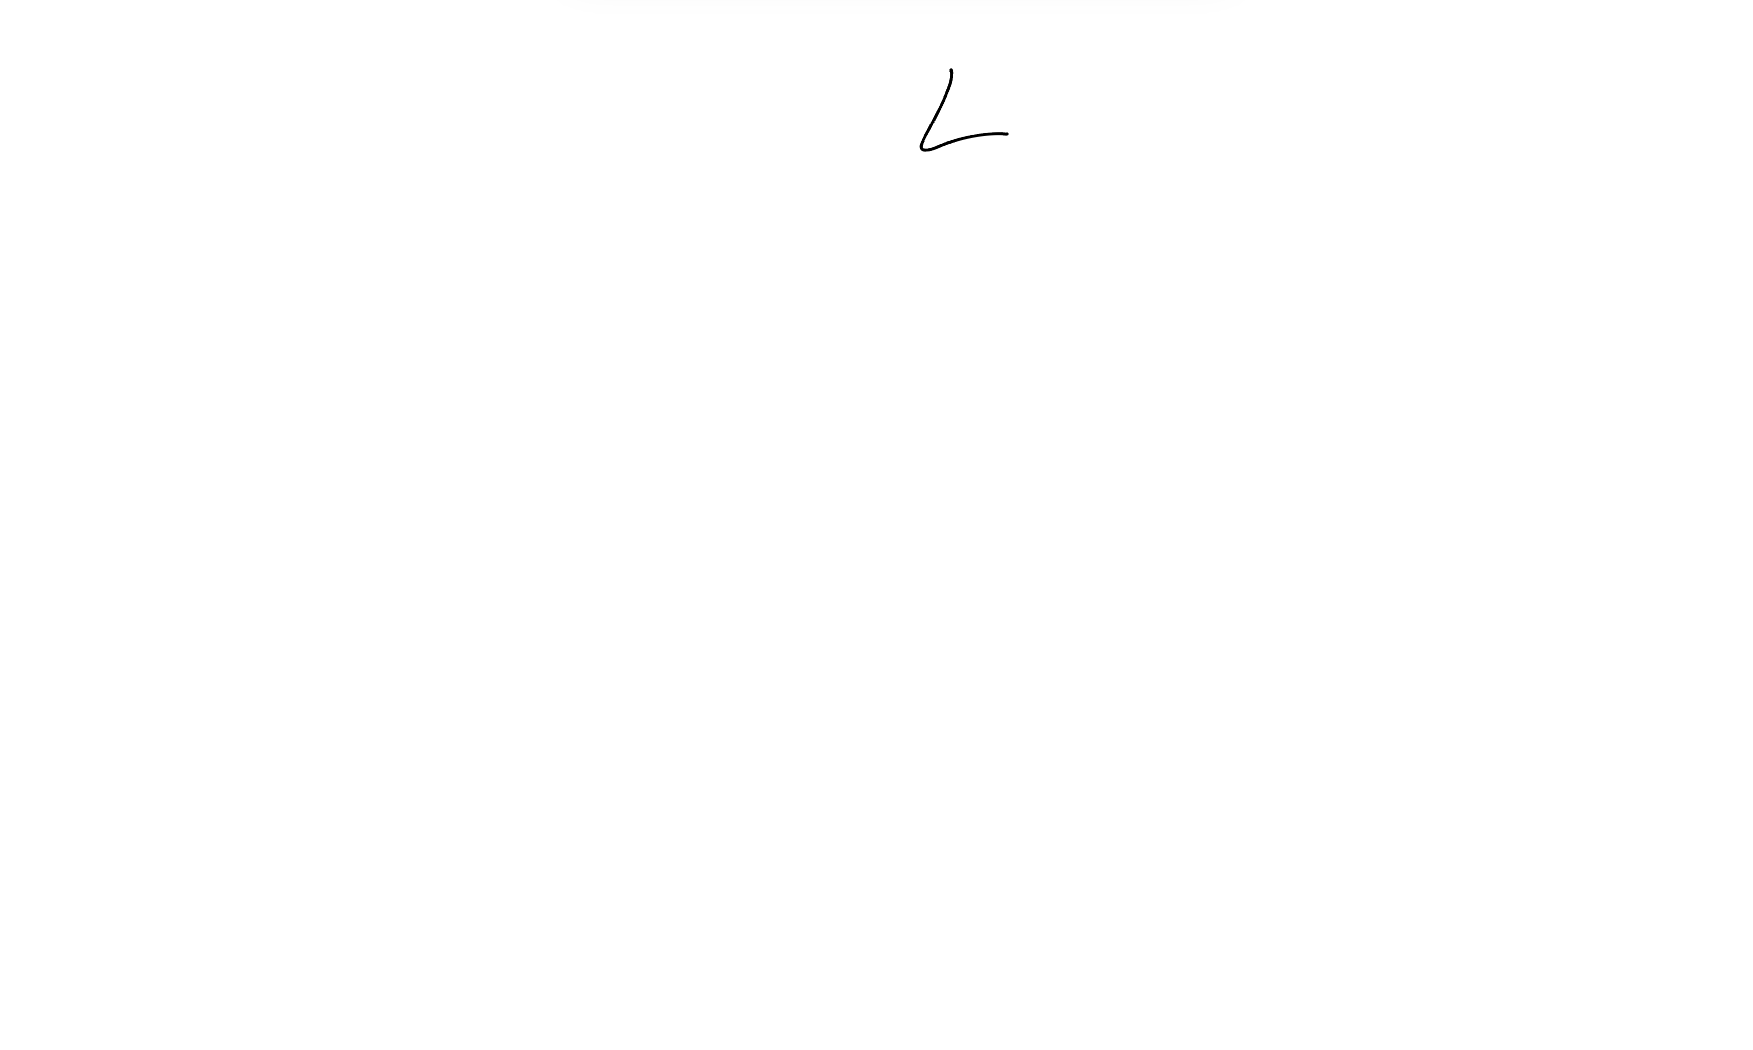
\includegraphics[scale=0.2]{Step1.PNG}
                \onslide<3>\centering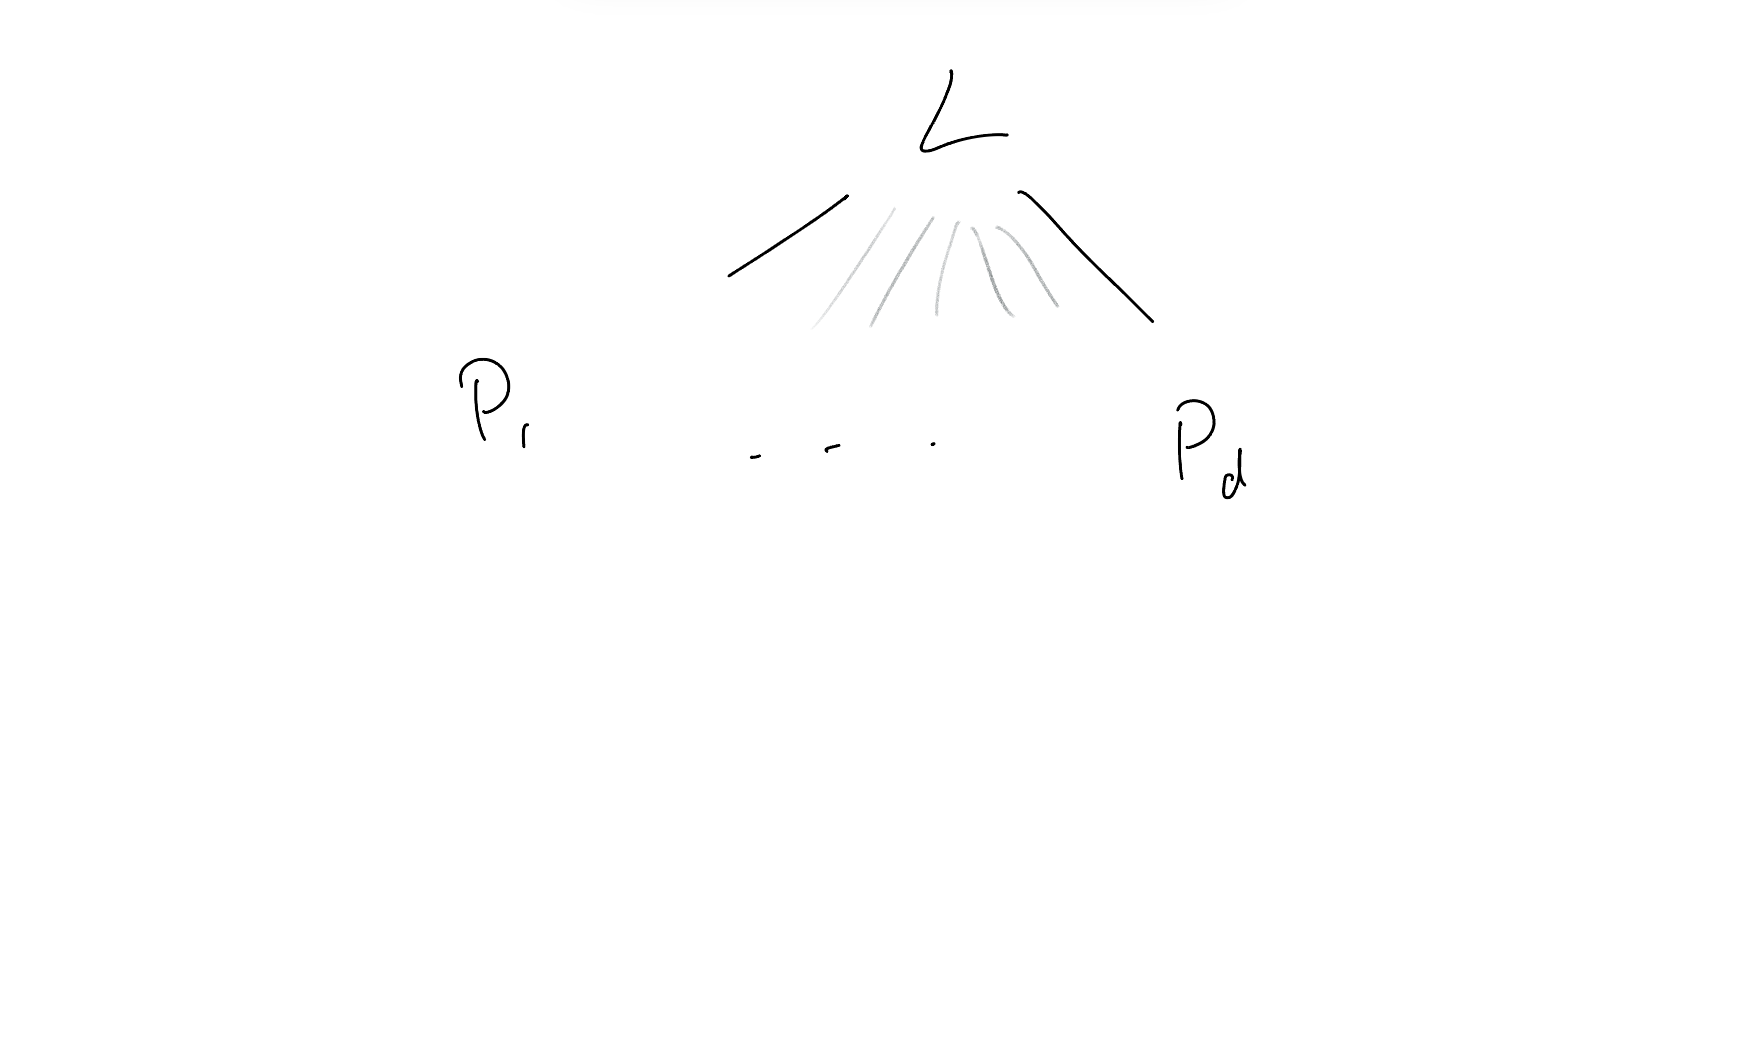
\includegraphics[scale=0.2]{Step2.PNG}
                \onslide<4>\centering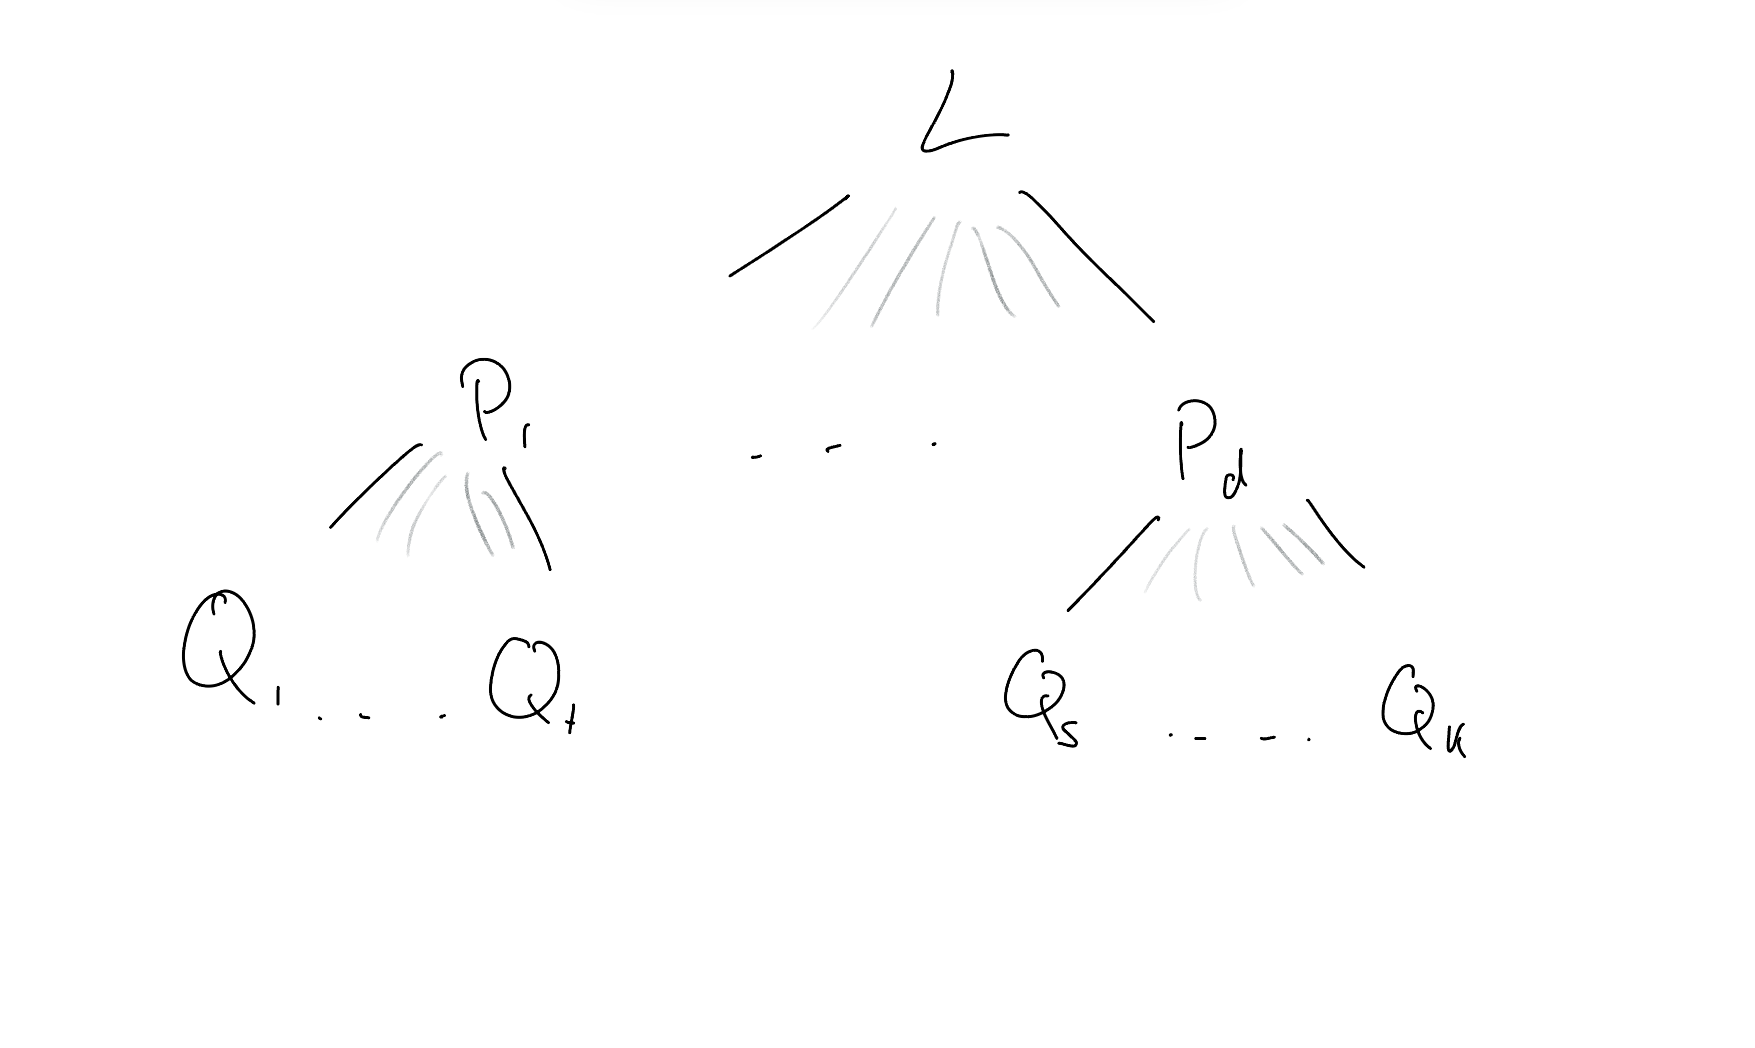
\includegraphics[scale=0.2]{Step3.PNG}
                \onslide<5>\centering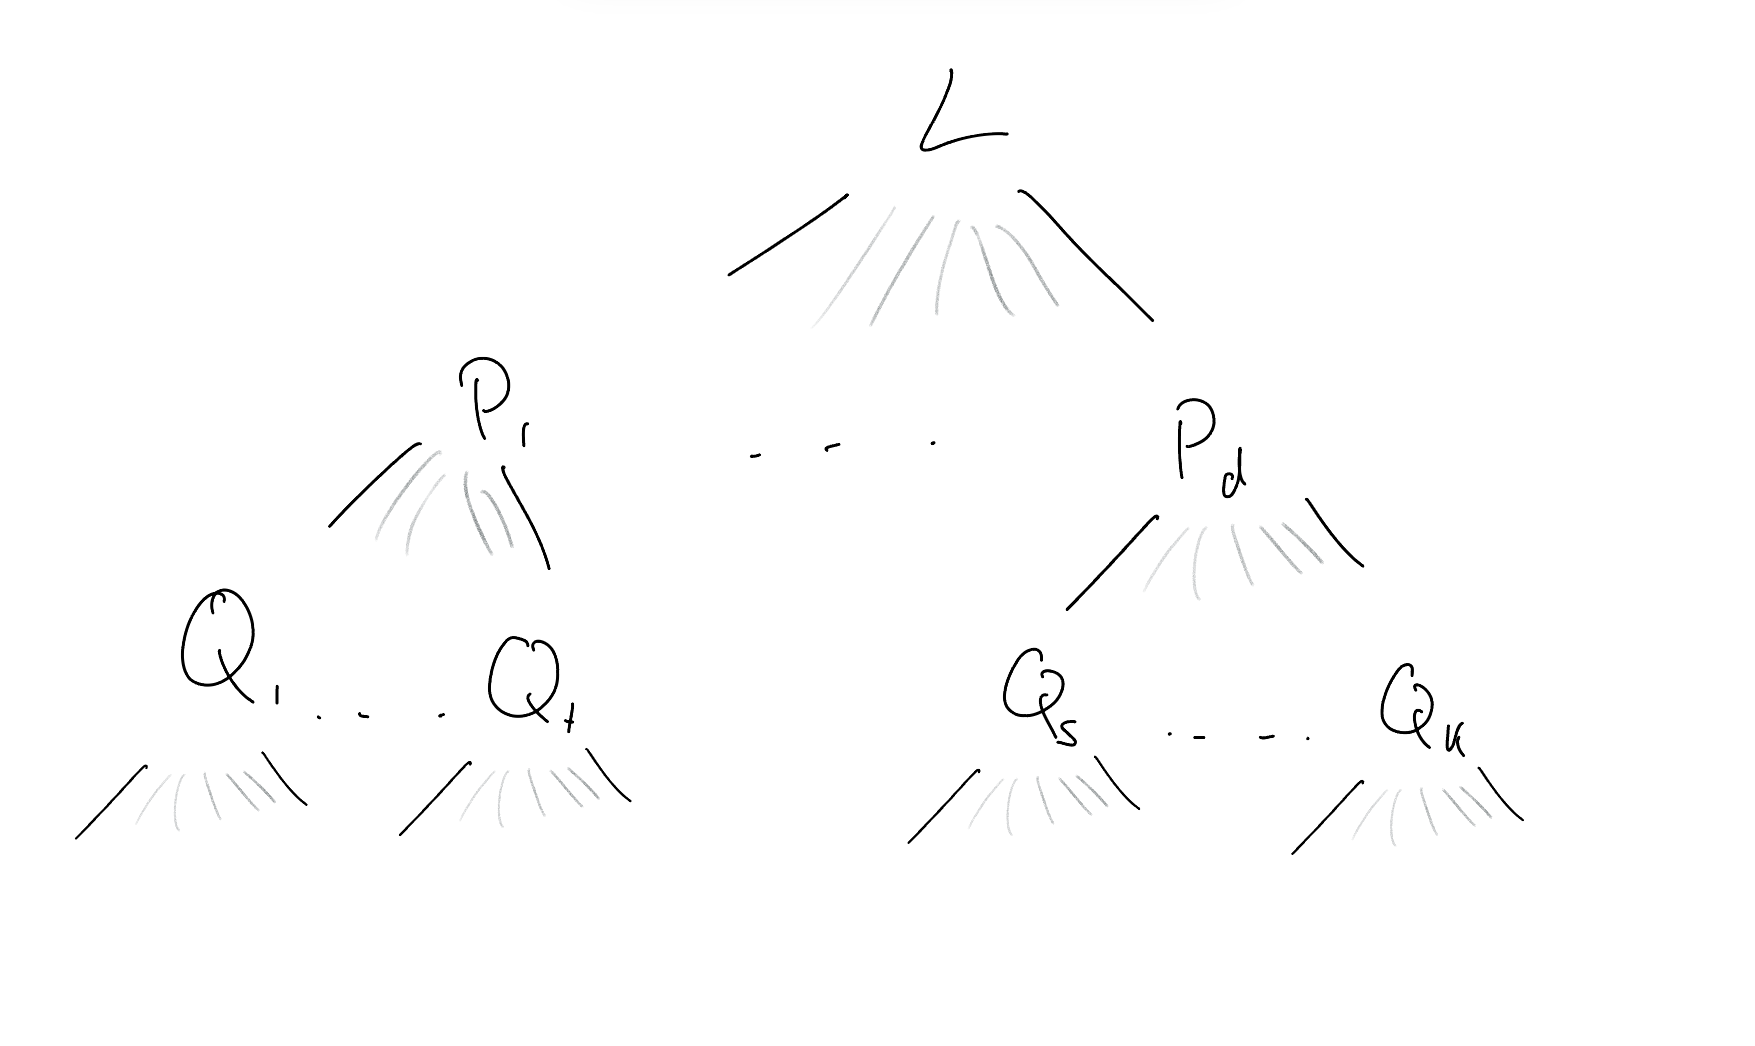
\includegraphics[scale=0.2]{Step4.PNG}
                \onslide<6->\centering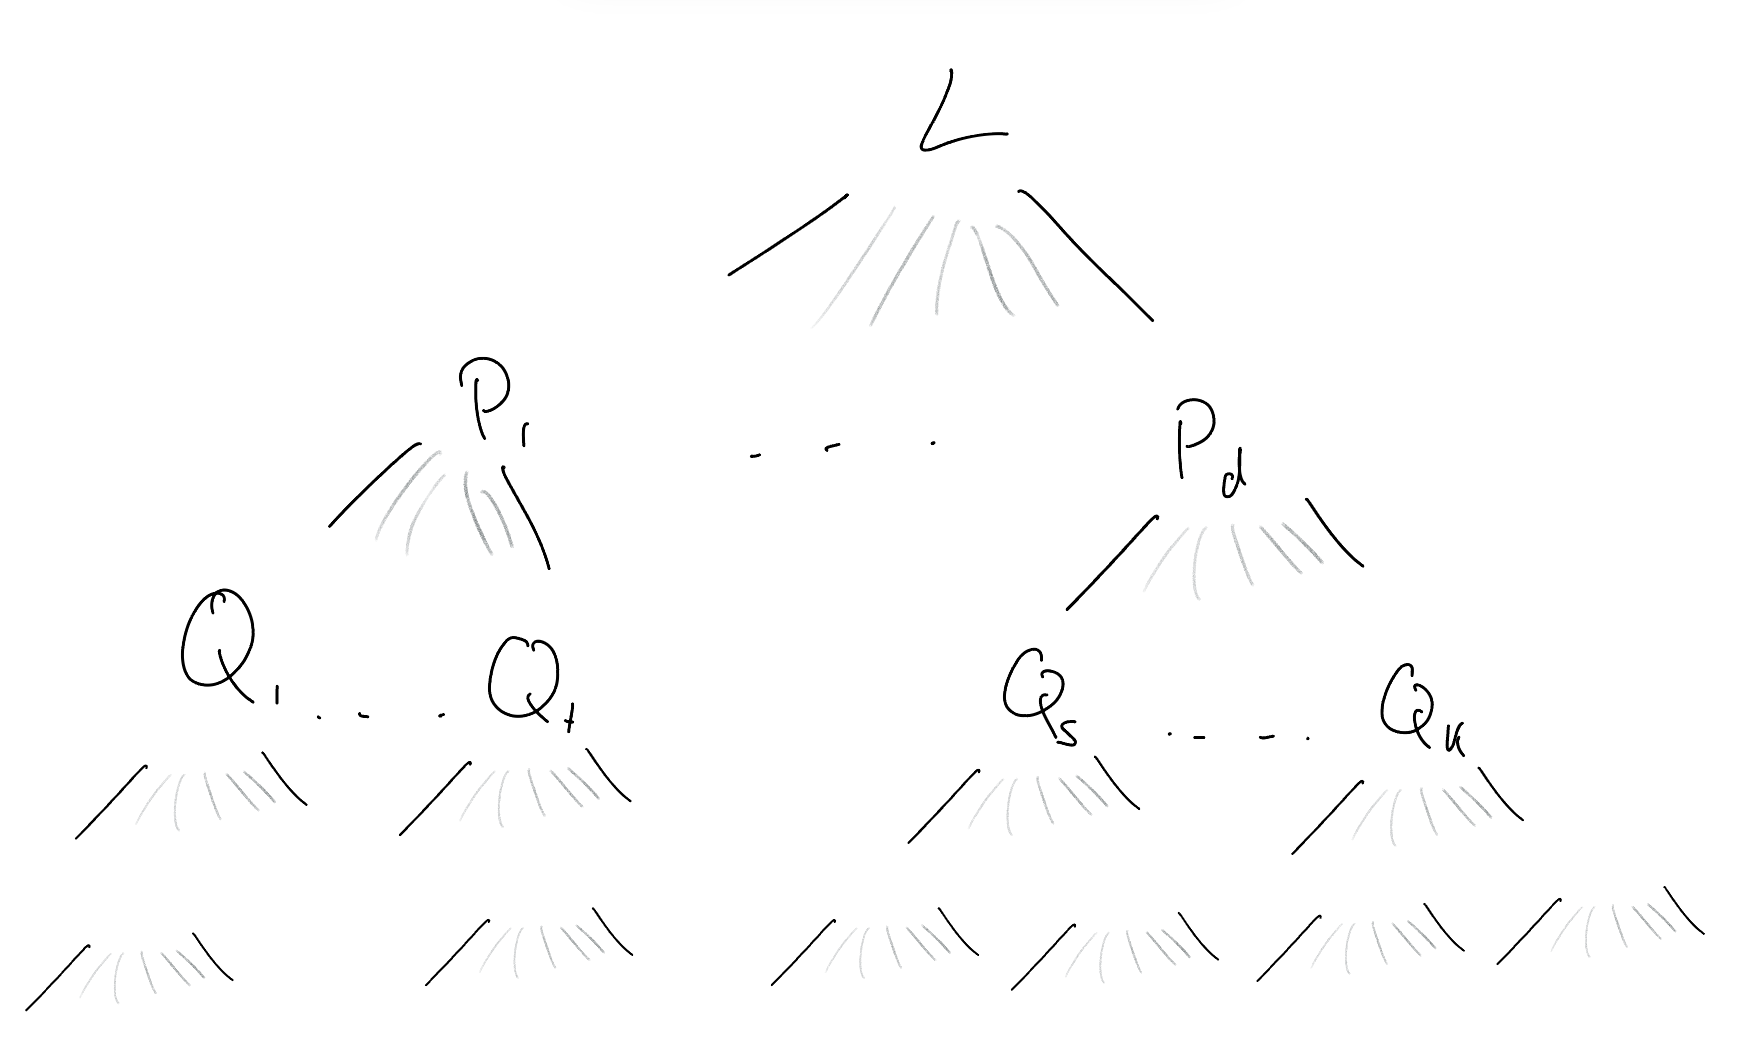
\includegraphics[scale=0.2]{Step5.PNG}
            \end{overprint}
        \end{figure}
        % \includegraphics[scale=0.2]{./Shortening.png}
    % \end{center}
\end{frame}

\begin{frame}
    \begin{block}{}
        This prosses must terminate!
        
        When it terminates, the subgroups has $\nb{\varphi_n}$ bounded (restricted to the corresponing subgroup)
    \end{block}

    \begin{corollary}
        $L$ is finitely presented by finitely many finitely subgroups $N_1, \ldots, N_l$ such that $\nb{\varphi_{n}\big\vert_{\tilde{N}_i}}$ is bounded for every $i$

        Thus $\varphi_n$ eventually factor through $G \onto L$
    \end{corollary}

    \begin{Theorem}
        If $\Gamma$ is a finitely generated hyperbolic group then $\Gamma$ is equationally noetherian.
    \end{Theorem}

\end{frame}

\begin{frame}
    \frametitle<overlay specification>[short title]{Hyperbolic-esque Groups}
    This procedure still apply is $\Gamma$ acts (with some assumptions) on hyperbolic space $X$. We still have the lemma
    \begin{lemma}
        $L$ is finitely presented by finitely many finitely subgroups $N_1, \ldots, N_l$ such that $\nb{\varphi_{n}\big\vert_{\tilde{N}_i}}$ is bounded for every $i$
    \end{lemma}

    Since $X$ is not the cayley graph we dont know that if $\nb{\varphi_n}$ is bounded then $\varphi_n$ eventually factor through $G\onto L$.
\end{frame}
\end{document}